%!TEX root = ../report.tex

\begin{document}
    \chapter{Experimental Setup}
    This chapter details the experimental setup used to train RandLA-Net for Deep Ensembles, Flipout and Dropout.

    % \section{Semantic segmentation model}
    % In this thesis, we used the RandLA-Net model for 3D semantic segmentation proposed in \cite{Hu_2020_CVPR_Randla}.
    % Section 2.1 describes the detailed working of RandLA-Net. 

    %\textcolor{red}{Merge this section to Datasets and Benchmarking chapter}
    %\section{Dataset}
    %In this thesis, we used Semantic3D as training dataset and more about the dataset is discussed in Section~\ref{sec:dataset_sem3d}.
    %Semantic3D is an ongoing benchmark challenge, so we evaluated our trained on the validation set.
    %For a sanity check, we cross-checked the performance of our trained models on this validation set with the pretrained model from the authors provided in \footnote[1]{https://github.com/QingyongHu/RandLA-Net}.

    \section{Training parameters}
    This section will discuss the libraries used and training parameters of the RandLA-Net for Deep Ensembles, and Flipout.    The training and testing of Deep Neural Networks are time and resource-intensive.
    We used the High-Performance Computing (HPC) GPU cluster from DFKI, especially on Nvidia Titan-XP and Nvidia-Tesla V100.
    \section{Libraries}
    With the purpose of reproducibility in mind, here we provide the list of major libraries used and their versions used for training.
    We also added the requirements.txt in the attached code for ease of reproduction as it is a struggle to set up the environment.
    \begin{enumerate}
        \item Python - 3.6
        \item Tensorflow - 1.15.0
        \item Tensorflow probability - 0.7.0
        \item Open3d-python - 0.3.0 (training), 0.13.0 (visualizations)
    \end{enumerate}
    
    \section{RandLA-Net - Deep Ensembles}
    \label{sec:de_setup}
    For Deep Ensembles, we trained 20 randomly initialized instances of RandLA-Net on the Semantic3D dataset.
    We used the default training parameters as provided by the authors, and they are a learning rate of 0.01 with the decay of 0.95 multiplied for every epoch, batch size of 4 and trained for 100 epochs.
    We changed the pipeline to infer the whole point cloud and save the probability scores from these 20 models.
    This change is made because the setup provided by authors infer only few points and then smoothen these softmax scores to the neighbouring points of inferred points.
    These saved probabilities from 20 models are averaged, and Maximum Softmax Probability (MSP) and Entropy are calculated.
    Out of these 20 models, we provide the evaluation for every $5^{th}$ model, i.e., 1, 5, 10, 15 and 20.
    \section{RandLA-Net - Flipout}
    \label{sec:flipout_setup}
    For Flipout-versioned RandLA-Net, we replaced the last three classification layers of the RandLA-Net highlighted with the red box in Figure~\ref{fig:fout_randlanet} with their Flipout counterparts from Tensorflow Probability.
    In addition to this change, we also removed the Dropout layer after the second classification layer.
    We chose these three layers because they are significant decision-makers for classification, and the remaining network is a feature extraction module.
    Following the same training procedure stated by the authors, we observed similar performance, so we decided not to change any training parameters.
    However, we initialized the Flipout weight perturbations with a normal prior of standard deviation 1.
    We also tried this with various standard deviations such as 0.1, 0.5, 1, 1.5, and 2.0 and found that standard deviation values of 0.5 and 1.0 result in better convergence.
    In comparison to Deep Ensembles, we performed 20 forward passes for the Flipout versioned RandLA-Net model, then averaged the results and represented every $5^{th}$ forward pass.
    \begin{figure}
        \centering
        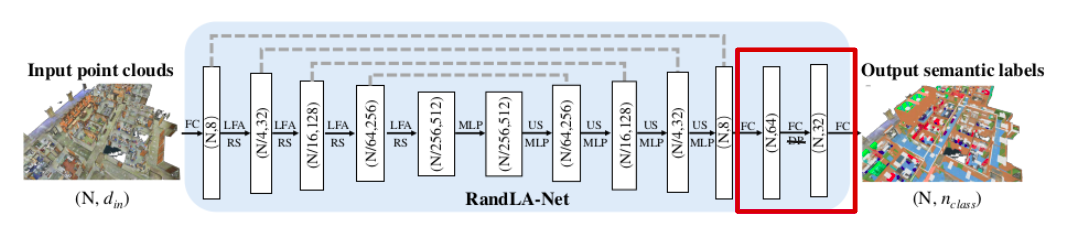
\includegraphics[scale=0.42]{images/fout_randlanet.png}
        \caption{Flipout-versioned RandLA-Net where the last three FC layers are made Flipout compatible represented in red box. Image taken from \cite{Hu_2020_CVPR_Randla}.}
        \label{fig:fout_randlanet}
    \end{figure}
    The Dropout version of the RandLA-Net setup is described in Section~\ref{sec:randladout} as it is only used for the evaluation of OOD detection more as a baseline method.
\end{document}
